% -------------------------------------------------------------------------------------------------
% SOLUTION ARCHITECTURE
% -------------------------------------------------------------------------------------------------
\section{Solution}
\label{sec:solution}
In this section we will describe the solution of work, i.e, Cloud4Things architecture:
% -------------------------------------------------------------------------------------------------
% DOCKER
% -------------------------------------------------------------------------------------------------
\subsection{Docker}
\label{sub:docker}
Docker\footnote{https://www.docker.com} is an open source project to pack, ship and run any application
as a lightweight container. Docker containers are \textit{hardware-agnostic} and \textit{platform-agnostic},
this means that these containers can run anywhere, from a laptop to a EC2 compute instance. Since that Docker
is based in Linux Containers (LXC), the virtualization is performed at operating-system level, different of
hypervisor-based solutions where the virtualization is performed at hardware-level. While the effect of both
types of virtualization are similar, the virtualization at the operating-system level provides significant
benefits compared to hypervisor-based solutions. Docker containers are small, they have basically zero
memory and CPU overhead, they also are completable portable between different virtualization environments.

In our solution, we are using Docker containers for provisioning the software stack of the Fosstrak platform.
A complete installation of the Fosstrak platform requires a compatible Java SDK, a full MySQL database and
a Apache Tomcat server. In order to improve the application scalability we are provisioning a single container 
for each component of the Fosstrak platform, the EPCIS repository, the Capture application, the ALE server,
and also for the MySQL database, as illustrated on Figure \ref{fig:docker_stack}.

% Dockerized application stack
\begin{figure}
  \centering
  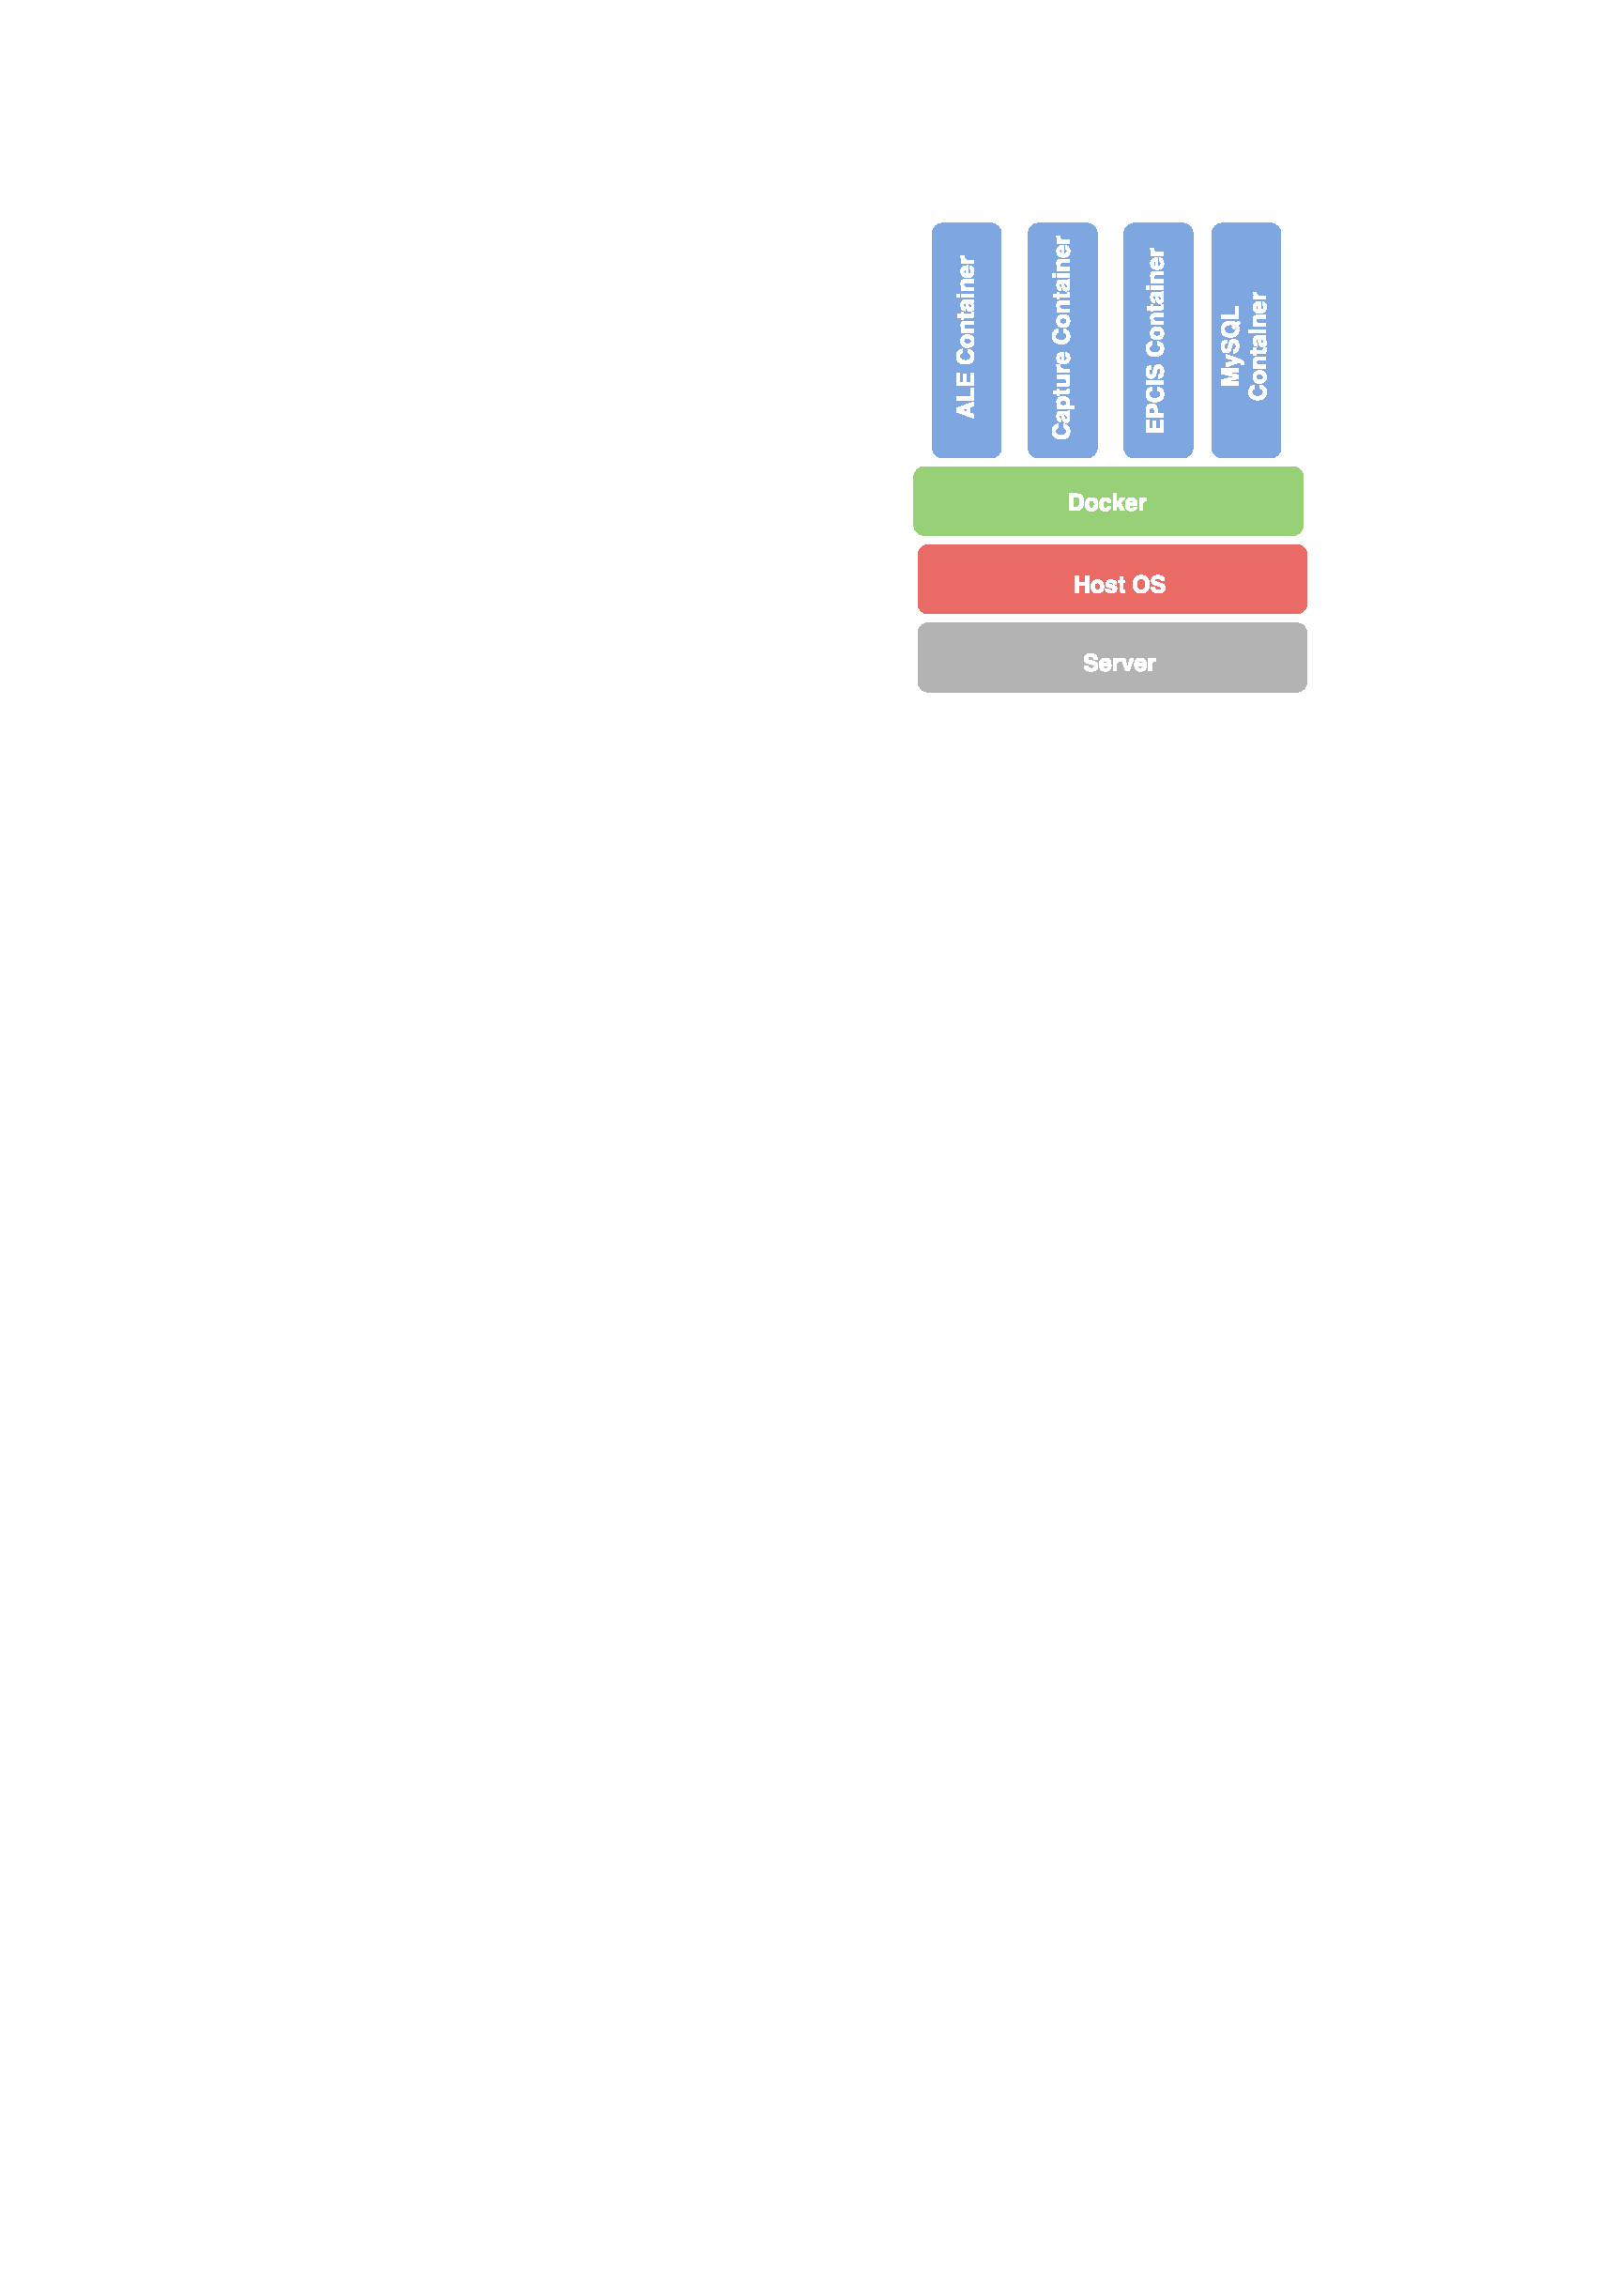
\includegraphics[width=.5\textwidth]{images/docker-stack}
  \caption{Docker-based application stack.}
  \label{fig:docker_stack}
\end{figure}

By default each container runs a process that is isolated from the other processes that are executed in the
same machine, inclusive the processes that runs in other containers. In order to connect the different
modules of the Fosstrak platform, our containers are linked through the \textit{linking} mechanism provided
by Docker.
% -------------------------------------------------------------------------------------------------
% AUTOMATIC PROVISIONING
% -------------------------------------------------------------------------------------------------
\subsection{Automatic Provisioning}
\label{sub:Automatic Provisioning}
In this section we will introduce the configuration management tools, in particular Chef, and then
we will present a detailed explanation about how we use Chef to perform the automatic provisioning
in the Cloud providers, in our case AWS, but by using Chef it is possible to port the
infrastructure to others providers.
\begin{figure}
  \centering
  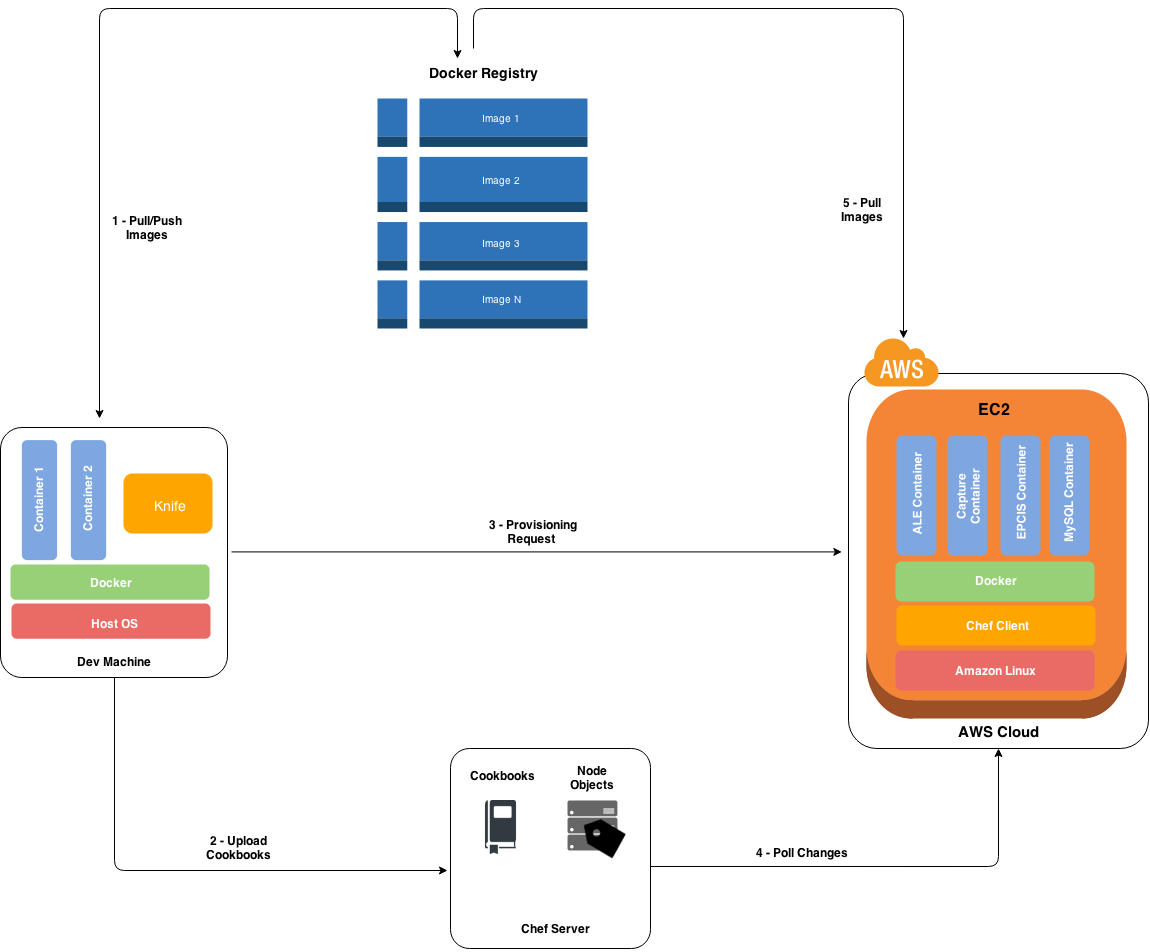
\includegraphics[width=.8\textwidth]{images/docker-c4t}
\end{figure}
% -------------------------------------------------------------------------------------------------
% SMART PLACE AUTOMATIC CONFIGURATION
% -------------------------------------------------------------------------------------------------
\subsection{Smart Place Automatic Configuration}
\label{sub:Smart Place Automatic Configuration}
In this section we will introduce the Cloud4Things CLI, a command line interface that allows the
users to upload a predefined configuration of a smart place to the Fosstrak server. We will explain
the procedures required to configure a smart place, i.e, the template that is used to describe the
configuration.
